\chapter{Arhitektura i dizajn sustava}
		
		\textbf{\textit{dio 1. revizije}}\\

		\textit{ Potrebno je opisati stil arhitekture te identificirati: podsustave, preslikavanje na radnu platformu, spremišta podataka, mrežne protokole, globalni upravljački tok i sklopovsko-programske zahtjeve. Po točkama razraditi i popratiti odgovarajućim skicama:}
	\begin{itemize}
		\item 	\textit{izbor arhitekture temeljem principa oblikovanja pokazanih na predavanjima (objasniti zašto ste baš odabrali takvu arhitekturu)}
		\item 	\textit{organizaciju sustava s najviše razine apstrakcije (npr. klijent-poslužitelj, baza podataka, datotečni sustav, grafičko sučelje)}
		\item 	\textit{organizaciju aplikacije (npr. slojevi frontend i backend, MVC arhitektura) }		
	\end{itemize}

	Arhitektura se moze podijeliti na tri podsustava:
	
	\begin{itemize}
		\item Web posluzitelj
		\item Web aplikacija
		\item Baza podataka
	\end{itemize}

	
	\textit{Web preglednik} je alat koji omogućava korisnicima pregledavanje web stranica i njihovih povezanih multimedijalnih sadržaja. Svaki internetski preglednik djeluje kao prevoditelj, jer interpretira web stranice napisane u kodu kako bi ih prikazao korisnicima na razumljiv način. Korisnici putem web preglednika šalju zahtjeve web poslužitelju.
	
	\textit{Web poslužitelj} je ključni element u radu web aplikacije. Njegova glavna uloga je olakšavanje komunikacije između klijenta i aplikacije putem HTTP protokola. Poslužitelj pokreće web aplikaciju i prenosi joj zahtjev.
	
	\textit{Web aplikacija} služi korisniku za obradu željenih zahtjeva. Aplikacija obrađuje zahtjev, pristupa bazi podataka prema potrebi i putem poslužitelja vraća korisniku odgovor u obliku HTML dokumenta koji se prikazuje u web pregledniku.
	
	\textit{Baza podataka} ima svrhu pohranjivanja i upravljanja strukturiranim podacima koji se koriste u aplikaciji. Svaki put kad korisnik šalje zahtjev putem web preglednika, web aplikacija može pristupiti bazi podataka kako bi dohvatila ili ažurirala potrebne informacije. Baza podataka omogućava učinkovit pristup, pretraživanje i manipulaciju podacima, što je ključno za pravilan rad web aplikacije.
	
	Za izradu naše web aplikacije odabrali smo programski jezik Java zajedno s Springboot radnim okvirom, kao i programski jezik JavaScript. Razvojna okruženja koja koristimo su Visual Studio Code i IntelliJ. Arhitektura sustava temelji se na MVC (Model-View-Controller) konceptu, koji je podržan od strane Springboot radnog okvira i nudi gotove predloške koji olakšavaju razvoj web aplikacije. Kao poslužitelja baze podataka smo koristili PostgreSQL.
	
	MVC koncept donosi neovisnost u razvoju pojedinih dijelova aplikacije, što olakšava testiranje, kao i dodavanje novih svojstava u sustav. Sastoji se od:
	
	\begin{itemize}
		\item \textbf{Model} - Središnja komponenta sustava koja predstavlja dinamičke strukture podataka neovisne o korisničkom sučelju. Upravlja podacima, logikom i pravilima aplikacije, te prima ulazne podatke od Controllera.
		\item \textbf{View} - Ovdje se prikazuju podaci, primjerice u obliku grafova. Moguća su različita sučelja za prikaz informacija, poput grafičkog ili tabličnog prikaza podataka.
		\item \textbf{Controller} - Prima ulaze i prilagođava ih za daljnju interakciju s Modelom ili Viewom. Upravlja korisničkim zahtjevima i temeljem njih izvodi daljnje interakcije s ostalim elementima sustava.
	\end{itemize}
		

		

				
		\section{Baza podataka}
				
				Za bazu podataka koristi se relacijska baza podataka koja se sastoji od relacija. Svaka relacija ima svoje ime i atribute. Vrste atributa koji se mogu nalaziti u relaciji su primarni ključ, strani ključ ili atribut s nekom informacijom vezanom za relaciju. Baza podataka sastoji se od relacija:
		
				\begin{packed_item}
					\item user
					\item istrazivac
					\item voditelj
					\item tragac
					\item admin
					\item akcija
					\item zahtjev
					\item postaja
					\item osposobljenost
					\item zivotinja
					\item komentar
					\item lokacija 
				\end{packed_item}
		
			\subsection{Opis tablica}
			


				U relaciju \textbf{user} pohranjuju se podaci o korisniku: \textit{id, ime, prezime, foto\textunderscore{}path, username, email, lozinka}. Primarni ključ je \textit{id}, i nema stranih ključeva. S atributom \textit{id} je u odnosu One-to-One s relacijom \textbf{admin}, s atributom \textit{id} je u odnosu One-to-One s relacijom \textbf{istrazivac}, s atributom \textit{id} je u odnosu One-to-One s relacijom \textbf{voditelj} i s atributom \textit{id} je u odnosu One-to-One s relacijom \textbf{tragac}.
				
				
				\begin{longtblr}[
					label=none,
					entry=none
					]{
						width = \textwidth,
						colspec={|X[6,l]|X[6, l]|X[20, l]|}, 
						rowhead = 1,
					} %definicija širine tablice, širine stupaca, poravnanje i broja redaka naslova tablice
					\hline \SetCell[c=3]{c}{\textbf{user}}	 \\ \hline[3pt]
					\SetCell{LightGreen}id & INT	&  	id korisnika 	\\ \hline
					ime	& VARCHAR &  ime korisnika 	\\ \hline 
					prezime & VARCHAR &  prezime korisnika  \\ \hline 
					foto\textunderscore{}path & VARCHAR	&  putanja do slike korisnika  \\ \hline 
					username & VARCHAR	&  korisničko ime  \\ \hline 
					email & VARCHAR	&  email korisnika  \\ \hline 
					lozinka & VARCHAR	&  lozinka korisnika spremljena kao hash  \\ \hline 
				\end{longtblr}
				
				
				U relaciju \textbf{admin} pohranjuju se podaci: \textit{id}. Primarni ključ i ujedno i strani ključ je \textit{id}. S atributom \textit{id} je u odnosu One-to-One s relacijom \textbf{user}, s atributom \textit{id} je u odnosu One-to-Many s relacijom \textbf{istrazivac} i s atributom \textit{id} je u odnosu One-to-Many s relacijom \textbf{voditelj}.
				
				
				\begin{longtblr}[
					label=none,
					entry=none
					]{
						width = \textwidth,
						colspec={|X[6,l]|X[6, l]|X[20, l]|}, 
						rowhead = 1,
					} %definicija širine tablice, širine stupaca, poravnanje i broja redaka naslova tablice
					\hline \SetCell[c=3]{c}{\textbf{admin}}	 \\ \hline[3pt]
					\SetCell{LightBlue} id & INT & id korisničkog računa admina 	\\ \hline
				\end{longtblr}
				
				U relaciju \textbf{istrazivac} pohranjuju se podaci: \textit{id, potvrdio}. Primarni ključ i ujedno i strani ključ je \textit{id} i također je strani ključ \textit{potvrdio}. S atributom \textit{id} je u odnosu One-to-One s relacijom \textbf{user}, s atributom \textit{potvrdio} je u odnosu Many-to-One s relacijom \textbf{admin} i s atributom \textit{id} je u odnosu One-to-Many s relacijom \textbf{akcija}.
				
				\begin{longtblr}[
					label=none,
					entry=none
					]{
						width = \textwidth,
						colspec={|X[6,l]|X[6, l]|X[20, l]|}, 
						rowhead = 1,
					} %definicija širine tablice, širine stupaca, poravnanje i broja redaka naslova tablice
					\hline \SetCell[c=3]{c}{\textbf{istrazivac}}	 \\ \hline[3pt]
					\SetCell{LightBlue}id & INT	&  	id korisničkog računa istraživača 	\\ \hline
					\SetCell{LightBlue}potvrdio	& INT &  id korisničkog računa admina koji je potvrdio istraživača 	\\ \hline  
				\end{longtblr}
			
				U relaciju \textbf{voditelj} pohranjuju se podaci: \textit{id, postaja\textunderscore{}id, potvrdio}. Primarni ključ i ujedno i strani ključ je \textit{id} i također je strani ključ \textit{potvrdio} i \textit{postaja\textunderscore{}id}. S atributom \textit{id} je u odnosu One-to-One s relacijom \textbf{user}, s atributom \textit{potvrdio} je u odnosu Many-to-One s relacijom \textbf{admin} i s atributom \textit{postaja\textunderscore{}id} je u odnosu One-to-One s relacijom \textbf{postaja}.
				
				\begin{longtblr}[
					label=none,
					entry=none
					]{
						width = \textwidth,
						colspec={|X[6,l]|X[6, l]|X[20, l]|}, 
						rowhead = 1,
					} %definicija širine tablice, širine stupaca, poravnanje i broja redaka naslova tablice
					\hline \SetCell[c=3]{c}{\textbf{voditelj}}	 \\ \hline[3pt]
					\SetCell{LightBlue}id & INT	&  	id korisničkog računa voditelja 	\\ \hline
					\SetCell{LightBlue}postaja\textunderscore{}id & INT	&  	id postaje koju vodi voditelj 	\\ \hline
					\SetCell{LightBlue}potvrdio	& INT &  id korisničkog računa admina koji je potvrdio voditelja 	\\ \hline
				\end{longtblr}
			
			U relaciju \textbf{tragac} pohranjuju se podaci: \textit{id, postaja\textunderscore{}id, osposobljenost\textunderscore{}id}. Primarni ključ i ujedno i strani ključ je \textit{id} i također je strani ključ \textit{postaja\textunderscore{}id} i \textit{osposobljenost\textunderscore{}id}. S atributom \textit{id} je u odnosu One-to-One s relacijom \textbf{user}, s atributom \textit{postaja\textunderscore{}id} je u odnosu Many-to-One s relacijom \textbf{postaja}, s atributom \textit{osposobljenost\textunderscore{}id} je u odnosu Many-to-One s relacijom \textbf{osposobljenost}, s atributom \textit{id} je u odnosu One-to-Many s relacijom \textbf{zahtjev} i  s atributom \textit{id} je u odnosu One-to-Many s relacijom \textbf{lokacija}.
			
				\begin{longtblr}[
					label=none,
					entry=none
					]{
						width = \textwidth,
						colspec={|X[10,l]|X[6, l]|X[20, l]|}, 
						rowhead = 1,
					} %definicija širine tablice, širine stupaca, poravnanje i broja redaka naslova tablice
					\hline \SetCell[c=3]{c}{\textbf{tragac}}	 \\ \hline[3pt]
					\SetCell{LightBlue}id & INT	&  	id korisničkog računa tragača 	\\ \hline
					\SetCell{LightBlue}postaja\textunderscore{}id & INT	&  	id postaje kojoj pripada 	\\ \hline
					\SetCell{LightBlue}osposobljenost\textunderscore{}id	& INT &  id osposobljenosti tragača 	\\ \hline  
				\end{longtblr}
			
			U relaciju \textbf{akcija} pohranjuju se podaci: \textit{id, zapoceo, opis}. Primarni ključ je \textit{id}, strani ključ je \textit{zapoceo}. S atributom \textit{zapoceo} je u odnosu Many-to-One s relacijom \textbf{istrazivac} i s atributom \textit{id} je u odnosu One-to-Many s relacijom \textbf{zahtjev}.
			
			\begin{longtblr}[
				label=none,
				entry=none
				]{
					width = \textwidth,
					colspec={|X[6,l]|X[6, l]|X[20, l]|}, 
					rowhead = 1,
				} %definicija širine tablice, širine stupaca, poravnanje i broja redaka naslova tablice
				\hline \SetCell[c=3]{c}{\textbf{akcija}}	 \\ \hline[3pt]
				\SetCell{LightGreen}id & INT	&  	id akcije 	\\ \hline
				\SetCell{LightBlue}zapoceo & INT	&  	id istraživača koji je započeo akciju 	\\ \hline
				opis	& TEXT &  opis akcije 	\\ \hline  
			\end{longtblr}
			
			U relaciju \textbf{zahtjev} pohranjuju se podaci: \textit{id, akcija\textunderscore{}id, tragac\textunderscore{}id, opis, kvalifikacije, zavrseno}. Primarni ključ je \textit{id}, strani ključevi su \textit{akcija\textunderscore{}id} i \textit{tragac\textunderscore{}id}. S atributom \textit{akcija\textunderscore{}id} je u odnosu Many-to-One s relacijom \textbf{akcija} i s atributom \textit{tragac\textunderscore{}id} je u odnosu Many-to-One s relacijom \textbf{tragac}.
			
			\begin{longtblr}[
				label=none,
				entry=none
				]{
					width = \textwidth,
					colspec={|X[6,l]|X[6, l]|X[20, l]|}, 
					rowhead = 1,
				} %definicija širine tablice, širine stupaca, poravnanje i broja redaka naslova tablice
				\hline \SetCell[c=3]{c}{\textbf{zahtjev}}	 \\ \hline[3pt]
				\SetCell{LightGreen}id & INT	&  	id zahtjeva 	\\ \hline
				\SetCell{LightBlue}akcija\textunderscore{}id & INT	&  	id akcije kojoj pripada zahtjev 	\\ \hline
				\SetCell{LightBlue}tragac\textunderscore{}id & INT	&  	id tragača koji je dobio zahtjev 	\\ \hline
				opis	& TEXT &  opis  što tragač mora napraviti 	\\ \hline 
				kvalifikacije & TEXT & koje su kvalifikacije potrebne \\ \hline
				zavrseno & BOOLEAN & je li zahtjev završen ili ne \\ \hline
			\end{longtblr}
			
			U relaciju \textbf{postaja} pohranjuju se podaci: \textit{id, ime}. Primarni ključ je \textit{id} i nema stranih ključeva. S atributom \textit{id} je u odnosu One-to-One s relacijom \textbf{voditelj}, s atributom \textit{id} je u odnosu One-to-Many s relacijom \textbf{tragac} i s atributom \textit{id} je u odnosu One-to-One s relacijom \textbf{lokacija}.
			
			\begin{longtblr}[
				label=none,
				entry=none
				]{
					width = \textwidth,
					colspec={|X[6,l]|X[6, l]|X[20, l]|}, 
					rowhead = 1,
				} %definicija širine tablice, širine stupaca, poravnanje i broja redaka naslova tablice
				\hline \SetCell[c=3]{c}{\textbf{postaja}}	 \\ \hline[3pt]
				\SetCell{LightGreen}id & INT	&  	id postaje 	\\ \hline
				ime & VARCHAR & ime postaje \\ \hline
			\end{longtblr}
			
			U relaciju \textbf{osposobljenost} pohranjuju se podaci: \textit{id, opis, podrucje\textunderscore{}pokrivanja, vidljivost}. Primarni ključ je \textit{id} i nema stranih ključeva. S atributom \textit{id} je u odnosu One-to-Many s relacijom \textbf{tragac}.
			
			\begin{longtblr}[
				label=none,
				entry=none
				]{
					width = \textwidth,
					colspec={|X[10,l]|X[6, l]|X[20, l]|}, 
					rowhead = 1,
				} %definicija širine tablice, širine stupaca, poravnanje i broja redaka naslova tablice
				\hline \SetCell[c=3]{c}{\textbf{osposobljenost}}	 \\ \hline[3pt]
				\SetCell{LightGreen}id & INT	&  	id osposobljenost 	\\ \hline
				opis & VARCHAR & opis osposobljenosti (npr. pješice, autom,...) \\ \hline
				podrucje\textunderscore{}pokrivanja & INT & područje pokriveno u metrima \\ \hline
				vidljivost & INT & ocjena vidljivosti na skali od 1 do 10 (1 je najgore, a 10 najbolje) \\ \hline
			\end{longtblr}
			
			U relaciju \textbf{zivotinja} pohranjuju se podaci: \textit{id, vrsta, komentar}. Primarni ključ je \textit{id} i nema stranih ključeva. S atributom \textit{id} je u odnosu One-to-Many s relacijom \textbf{lokacija}.
			
			\begin{longtblr}[
				label=none,
				entry=none
				]{
					width = \textwidth,
					colspec={|X[6,l]|X[6, l]|X[20, l]|}, 
					rowhead = 1,
				} %definicija širine tablice, širine stupaca, poravnanje i broja redaka naslova tablice
				\hline \SetCell[c=3]{c}{\textbf{zivotinja}}	 \\ \hline[3pt]
				\SetCell{LightGreen}id & INT	&  	id životinje 	\\ \hline
				vrsta & VARCHAR & vrsta životinje \\ \hline
				komentar & TEXT & komentar za životinju \\ \hline
			\end{longtblr}
			
			U relaciju \textbf{komentar} pohranjuju se podaci: \textit{id, komentar}. Primarni ključ je \textit{id} i nema stranih ključeva. S atributom \textit{id} je u odnosu One-to-One s relacijom \textbf{lokacija}.
			
			\begin{longtblr}[
				label=none,
				entry=none
				]{
					width = \textwidth,
					colspec={|X[6,l]|X[6, l]|X[20, l]|}, 
					rowhead = 1,
				} %definicija širine tablice, širine stupaca, poravnanje i broja redaka naslova tablice
				\hline \SetCell[c=3]{c}{\textbf{komentar}}	 \\ \hline[3pt]
				\SetCell{LightGreen}id & INT	&  	id komentara 	\\ \hline
				komentar & TEXT & komentar za lokaciju \\ \hline
			\end{longtblr}
			
			
			U relaciju \textbf{lokacija} pohranjuju se podaci: \textit{objekt\textunderscore{}id, geo\textunderscore{}duzina, geo\textunderscore{}sirina, vrijeme}. Strani ključ je \textit{objekt\textunderscore{}id}. S atributom \textit{objekt\textunderscore{}id} je u odnosu One-to-One s relacijom \textbf{postaja}, One-to-One s relacijom \textbf{komentar}, Many-to-One s relacijom \textbf{zivotinja} i Many-to-One s relacijom \textbf{tragac}.
			
			\begin{longtblr}[
				label=none,
				entry=none
				]{
					width = \textwidth,
					colspec={|X[6,l]|X[6, l]|X[20, l]|}, 
					rowhead = 1,
				} %definicija širine tablice, širine stupaca, poravnanje i broja redaka naslova tablice
				\hline \SetCell[c=3]{c}{\textbf{lokacija}}	 \\ \hline[3pt]
				\SetCell{LightBlue}objekt\textunderscore{}id & INT	&  	id objekta na određenoj lokaciji 	\\ \hline
				geo\textunderscore{}duzina & DOUBLE & geografska dužina \\ \hline
				geo\textunderscore{}sirina & DOUBLE & geografska širina \\ \hline
				vrijeme & TIMESTAMP & vrijeme kada je lokacija spremljena \\ \hline
			\end{longtblr}
			
			\subsection{Dijagram baze podataka}
				\begin{figure}[H]
					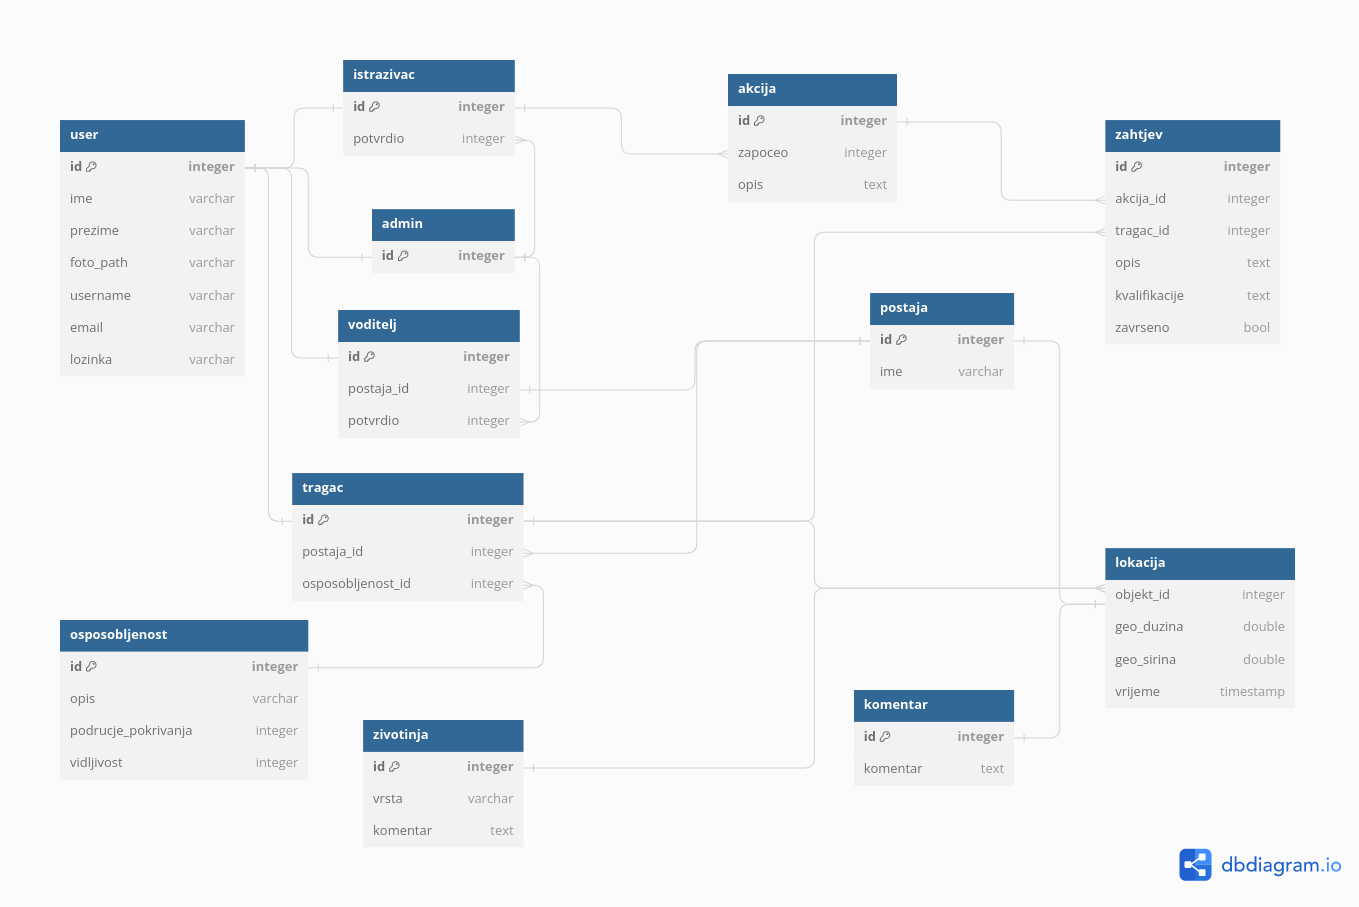
\includegraphics[scale=0.35]{slike/dijagram_baze_podataka.png}
					\centering
					\caption{Dijagram baze podataka}
					\label{fig:promjene}
				\end{figure}
			\eject
			
			
		\section{Dijagram razreda}
		
			\textit{Potrebno je priložiti dijagram razreda s pripadajućim opisom. Zbog preglednosti je moguće dijagram razlomiti na više njih, ali moraju biti grupirani prema sličnim razinama apstrakcije i srodnim funkcionalnostima.}\\
			
			\textbf{\textit{dio 1. revizije}}\\
			
			\textit{Prilikom prve predaje projekta, potrebno je priložiti potpuno razrađen dijagram razreda vezan uz \textbf{generičku funkcionalnost} sustava. Ostale funkcionalnosti trebaju biti idejno razrađene u dijagramu sa sljedećim komponentama: nazivi razreda, nazivi metoda i vrste pristupa metodama (npr. javni, zaštićeni), nazivi atributa razreda, veze i odnosi između razreda.}\\
			
			\textbf{\textit{dio 2. revizije}}\\			
			
			\textit{Prilikom druge predaje projekta dijagram razreda i opisi moraju odgovarati stvarnom stanju implementacije}
			
			
			
			\eject
		
		\section{Dijagram stanja}
			
			
			\textbf{\textit{dio 2. revizije}}\\
			
			\textit{Potrebno je priložiti dijagram stanja i opisati ga. Dovoljan je jedan dijagram stanja koji prikazuje \textbf{značajan dio funkcionalnosti} sustava. Na primjer, stanja korisničkog sučelja i tijek korištenja neke ključne funkcionalnosti jesu značajan dio sustava, a registracija i prijava nisu. }
			
			
			\eject 
		
		\section{Dijagram aktivnosti}
			
			\textbf{\textit{dio 2. revizije}}\\
			
			 \textit{Potrebno je priložiti dijagram aktivnosti s pripadajućim opisom. Dijagram aktivnosti treba prikazivati značajan dio sustava.}
			
			\eject
		\section{Dijagram komponenti}
		
			\textbf{\textit{dio 2. revizije}}\\
		
			 \textit{Potrebno je priložiti dijagram komponenti s pripadajućim opisom. Dijagram komponenti treba prikazivati strukturu cijele aplikacije.}